
\documentclass{standalone}
\usepackage{xcolor}
\usepackage{pgfplots}
\pgfplotsset{compat=1.18}

\begin{document}

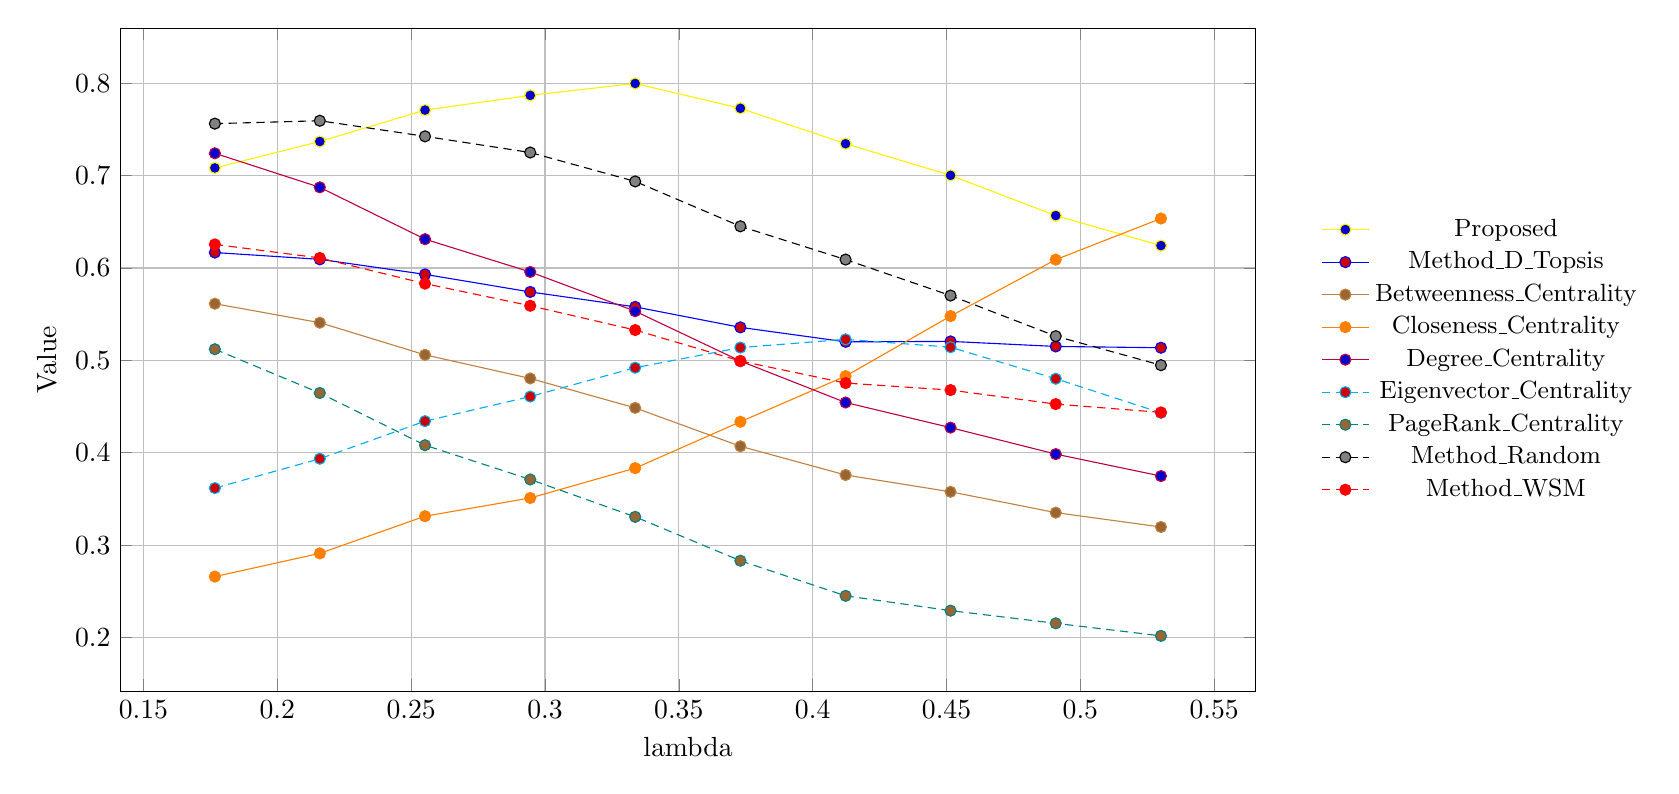
\begin{tikzpicture}
\begin{axis}[
    width=16cm,
    height=10cm,
    xlabel={lambda},
    ylabel={Value},
    grid=major,
    legend style={
        at={(1.05,0.5)},
        anchor=west,
        font=\small,
        draw=none,
        cells={align=left},
    },
]
% Proposed
\addplot+[color=yellow, mark=*] coordinates {
(0.1767,0.7083207976608319) (0.2159,0.7369139675699206) (0.2552,0.7709351245764181) (0.2945,0.7868600306499908) (0.3337,0.7997427090958514) (0.373,0.7728534678398464) (0.4123,0.7345396284615479) (0.4515,0.7002783934360701) (0.4908,0.6567032187902243) (0.5301,0.6242473972022056) };
\addlegendentry{Proposed}

% Method\_D\_Topsis
\addplot+[color=blue, mark=*] coordinates {
(0.1767,0.6167206944158058) (0.2159,0.6093675429549845) (0.2552,0.5930888702616551) (0.2945,0.574067102218375) (0.3337,0.5578973965272671) (0.373,0.5357331887598293) (0.4123,0.5200643076439574) (0.4515,0.5205292419291228) (0.4908,0.5150747229443352) (0.5301,0.5136799293817816) };
\addlegendentry{Method\_D\_Topsis}

% Betweenness\_Centrality
\addplot+[color=brown, mark=*] coordinates {
(0.1767,0.5613187973251521) (0.2159,0.5407941538614665) (0.2552,0.5059709999315272) (0.2945,0.4804348841085483) (0.3337,0.4485649077606545) (0.373,0.4070170131943749) (0.4123,0.3759292573510074) (0.4515,0.3577434068901464) (0.4908,0.3351861688552275) (0.5301,0.3196484955618803) };
\addlegendentry{Betweenness\_Centrality}

% Closeness\_Centrality
\addplot+[color=orange, mark=*] coordinates {
(0.1767,0.2659540699452805) (0.2159,0.2910733707819367) (0.2552,0.3313459916869763) (0.2945,0.3510299384998365) (0.3337,0.3833328081126085) (0.373,0.4335463571059443) (0.4123,0.4829525115887262) (0.4515,0.5479285016822337) (0.4908,0.6090519488131478) (0.5301,0.653565388422634) };
\addlegendentry{Closeness\_Centrality}

% Degree\_Centrality
\addplot+[color=purple, mark=*] coordinates {
(0.1767,0.7241490970402445) (0.2159,0.6873046027004516) (0.2552,0.631184570503453) (0.2945,0.5957025059384159) (0.3337,0.5532296967227812) (0.373,0.4992516541692509) (0.4123,0.4543984416305024) (0.4515,0.4272010363447814) (0.4908,0.3985310542829924) (0.5301,0.3747662653850272) };
\addlegendentry{Degree\_Centrality}

% Eigenvector\_Centrality
\addplot+[color=cyan, mark=*] coordinates {
(0.1767,0.3617486459179826) (0.2159,0.3935539732236514) (0.2552,0.4342088839752283) (0.2945,0.4608327127634967) (0.3337,0.4920598581445805) (0.373,0.5138493482779837) (0.4123,0.5227682751710534) (0.4515,0.5142174538455063) (0.4908,0.4801266136003373) (0.5301,0.4432276156535485) };
\addlegendentry{Eigenvector\_Centrality}

% PageRank\_Centrality
\addplot+[color=teal, mark=*] coordinates {
(0.1767,0.5120659614812553) (0.2159,0.4646944681306289) (0.2552,0.4081510152420511) (0.2945,0.371057097891439) (0.3337,0.3306127287222593) (0.373,0.2831358712098221) (0.4123,0.2451093754834454) (0.4515,0.2290916122039004) (0.4908,0.2153791209365243) (0.5301,0.2017893204663974) };
\addlegendentry{PageRank\_Centrality}

% Method\_Random
\addplot+[color=black, mark=*] coordinates {
(0.1767,0.7562456855826014) (0.2159,0.7593837537715676) (0.2552,0.7424950625468066) (0.2945,0.7250101974933258) (0.3337,0.6937062954519893) (0.373,0.645133684828961) (0.4123,0.6090969140550576) (0.4515,0.5701631240510574) (0.4908,0.5262082967106247) (0.5301,0.4948024098104865) };
\addlegendentry{Method\_Random}

% Method\_WSM
\addplot+[color=red, mark=*] coordinates {
(0.1767,0.6255522910350354) (0.2159,0.6108553058693997) (0.2552,0.5830599559304696) (0.2945,0.5591091509122309) (0.3337,0.5328202270464154) (0.373,0.4992683613286505) (0.4123,0.4754482603392635) (0.4515,0.4678433760008288) (0.4908,0.4526667260123366) (0.5301,0.4436900861638354) };
\addlegendentry{Method\_WSM}


\end{axis}
\end{tikzpicture}

\end{document}
